\chapter{Attacking Active Directory Group Managed Service Accounts (GMSAs)}

This post is meant to highlight what GMSAs can do and what an attacker can do if not protected appropriately. We have seen limited usage of Group Managed Service Accounts in AD environments when we perform Active Directory Security Assessments at Trimarc. GMSAs should be used wherever possible to replace user accounts as service accounts since the passwords will rotate automatically.

Group Managed Service Accounts (GMSAs)
User accounts created to be used as service accounts rarely have their password changed. Group Managed Service Accounts (GMSAs) provide a better approach (starting in the Windows 2012 timeframe). The password is managed by AD and automatically changed. This means that the GMSA has to have security principals explicitly delegated to have access to the clear-text password. Much like with other areas where delegation controls access (LAPS), determining who should have be delegated access needs to be be carefully considered.

Key Points for Group Managed Service Accounts (GMSAs) :

The GMSA password managed by AD.
Computers hosting GMSA service account(s) request current password from Active Directory to start service.
Configure the GMSA to allow computer accounts access to password.
If an attacker compromises computer hosting services using GMSA, the GMSA is compromised.
If attacker compromises an account with rights to request GMSA password, the GMSA is compromised.
Group Managed Service Accounts have the object class “msDS-GroupManagedServiceAccount” and associated attributes specific to GMSAs. These properties include:

msDS-GroupMSAMembership (PrincipalsAllowedToRetrieveManagedPassword) – stores the security principals that can access the GMSA password.
msds-ManagedPassword – This attribute contains a BLOB with password information for group-managed service accounts.
msDS-ManagedPasswordId – This constructed attribute contains the key identifier for the current managed password data for a group MSA.
msDS-ManagedPasswordInterval – This attribute is used to retrieve the number of days before a managed password is automatically changed for a group MSA.

\begin{figure}
    \centering
    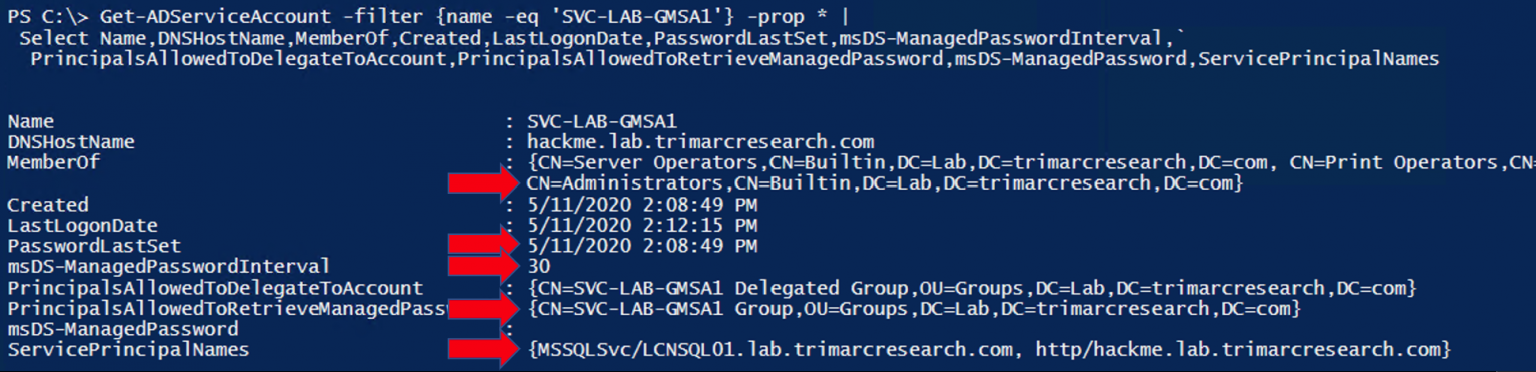
\includegraphics[width=0.75\linewidth]{msdspass.png}
    \caption{Enter Caption}
    \label{fig:placeholder}
\end{figure}

Running the AD PowerShell cmdlet Get-ADServiceAccount, we can retrieve information about the GMSA, including specific GMSA attrbiutes. This GMSA is a member of the domain Administrators group which has full AD \& DC admin rights to the domain. The screenshot shows that the password changed recently and won’t change for a few weeks – changed on 5/11/2020 and configured to change every 30 days. This means that if we can get the password for this account, we have almost a month to use the account credentials before it changes. We can also identify a group that can retrieve the password data. We’ll take a look at this is a bit.

Gaining Access to a Server Running a Service as a Group Managed Service Account

Once we get on the server/servers running services under the context of the GMSA we have some options. Let’s take a look…

\begin{figure}
    \centering
    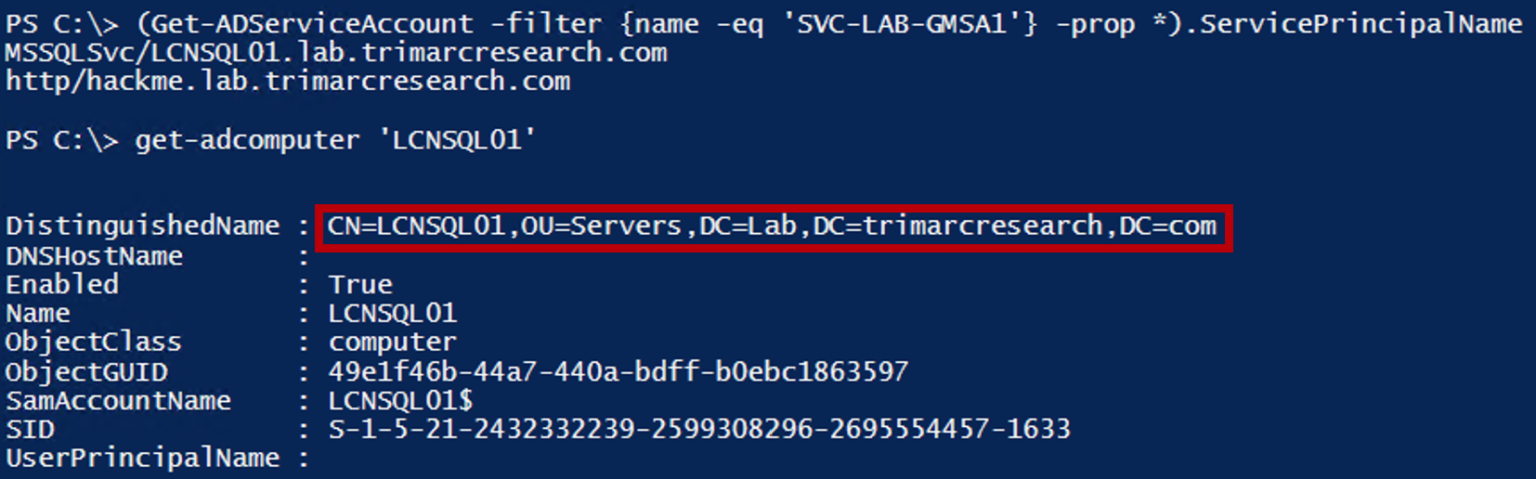
\includegraphics[width=0.75\linewidth]{srvcacct.png}
    \caption{Enter Caption}
    \label{fig:placeholder}
\end{figure}

We can identify the LCNSQL01 server is registered as a Service Principal Name (SPN) on the GMSA and we see this server is in the Servers OU.

If we can compromise an account with rights to the Servers OU, or delegated admin rights via GPO Restricted Groups or similar, or have the ability to modify a GPO that links to this OU, we can we can get admin rights on the LCN server
\begin{figure}
    \centering
    
\includegraphics[width=0.75\linewidth]{lcnsrv.png}
    \caption{Enter Caption}
    \label{fig:placeholder}
\end{figure}

After getting admin rights on the server associated with the GMSA, we can see there is a service running under the context of the GMSA (I cheated here and configured Windows License Manager Service to start with this account).

\begin{figure}
    \centering
    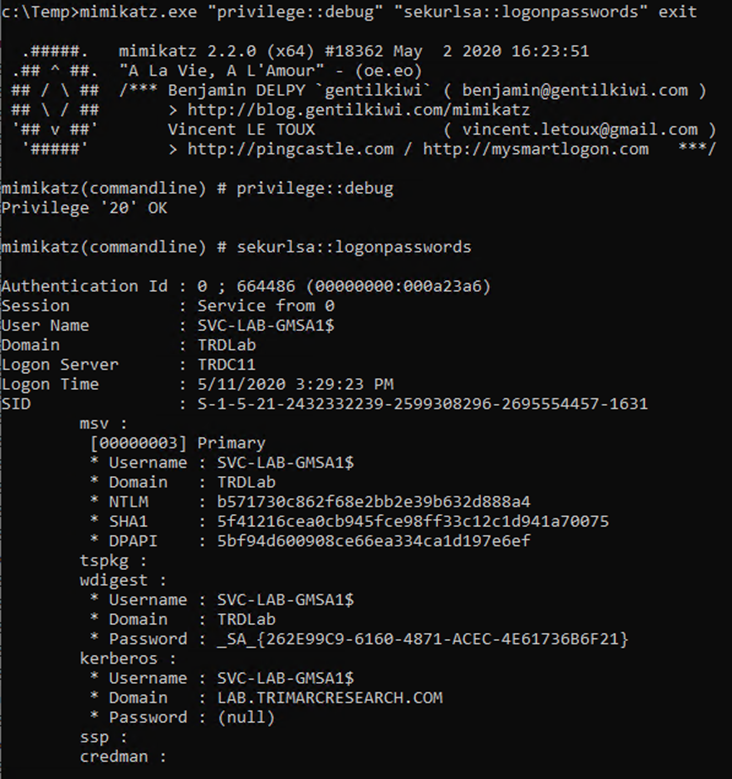
\includegraphics[width=0.75\linewidth]{acct.png}
    \caption{Enter Caption}
    \label{fig:placeholder}
\end{figure}

Since there’s a service running under the context of an account, we can get the password data associated with the service account. Here we use Mimikatz to dump LSASS using sekurlsa::logonpasswords.

That’s interesting, the password looks a bit unusual: “\_SA\_{262E99C9-6160-4871-ACEC-4E61736B6F21}”

That’s not a standard password (and not actually the one associated with the account). What’s more, this password hash isn’t correct. Microsoft loads the GMSA credential into LSASS but doesn’t seem to use it.

To get the right NT password hash we need to use the Mimikatz command “Sekurlsa::ekeys” which is what’s used to get Kerberos tickets.

\begin{figure}
    \centering
    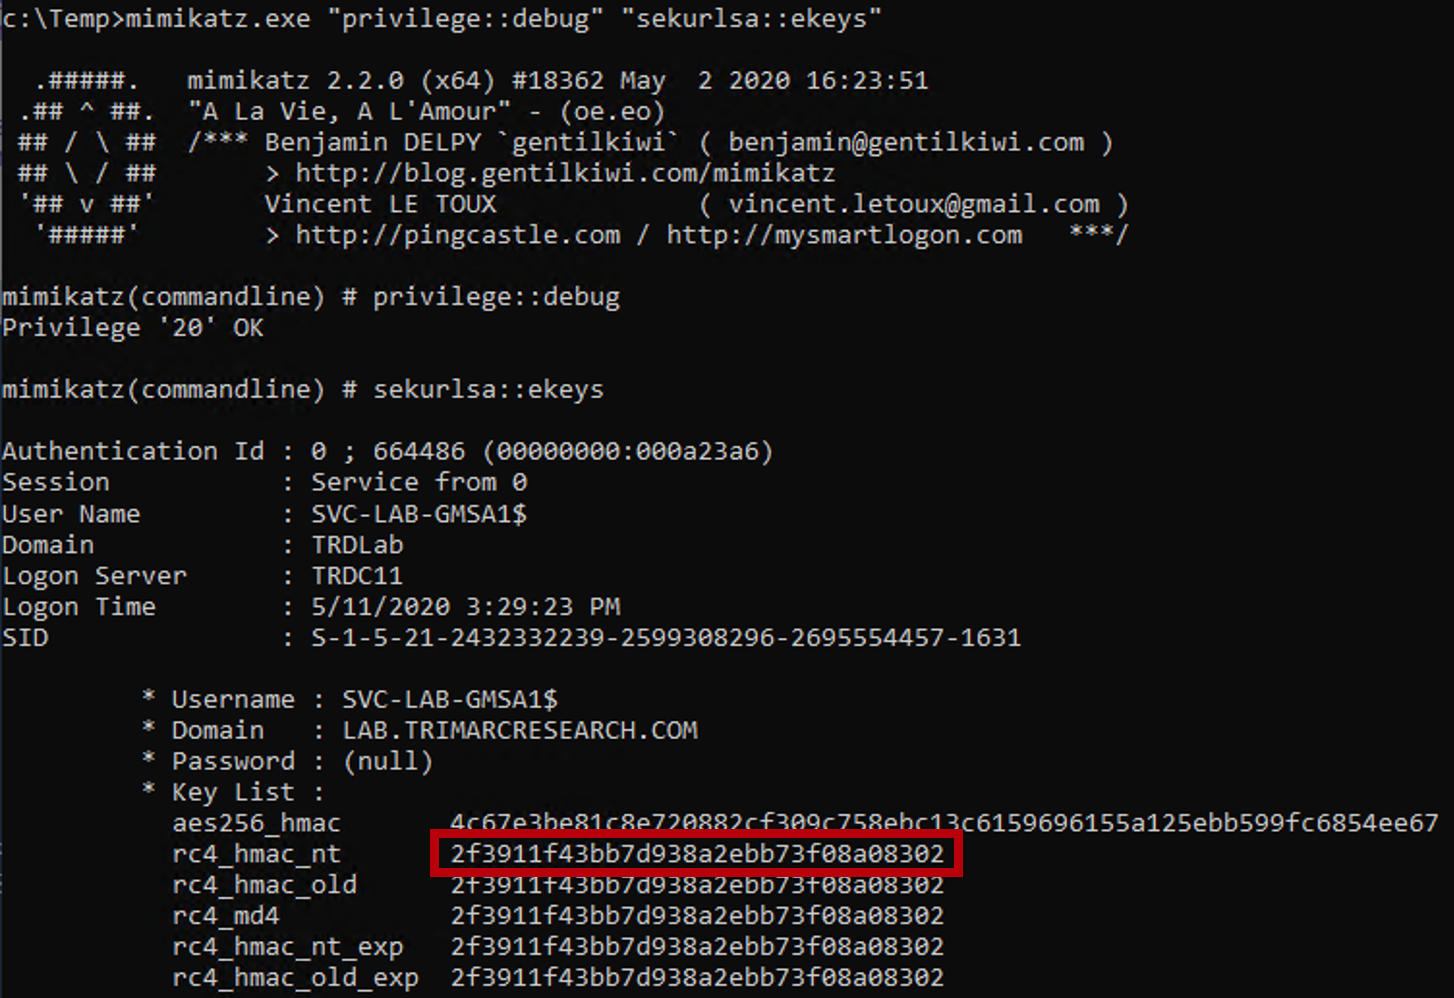
\includegraphics[width=0.75\linewidth]{mimi.png}
    \caption{Enter Caption}
    \label{fig:placeholder}
\end{figure}

After running this Mimikatz command, we are able to see password hash. With this password hash, we can pass the hash (PTH) to compromise AD.

But what if we couldn’t get access to the server itself?

Compromising an Account with GMSA Password Access
We know there is a group configured with rights to get the GMSA password, let’s take a look at that.

\begin{figure}
    \centering
    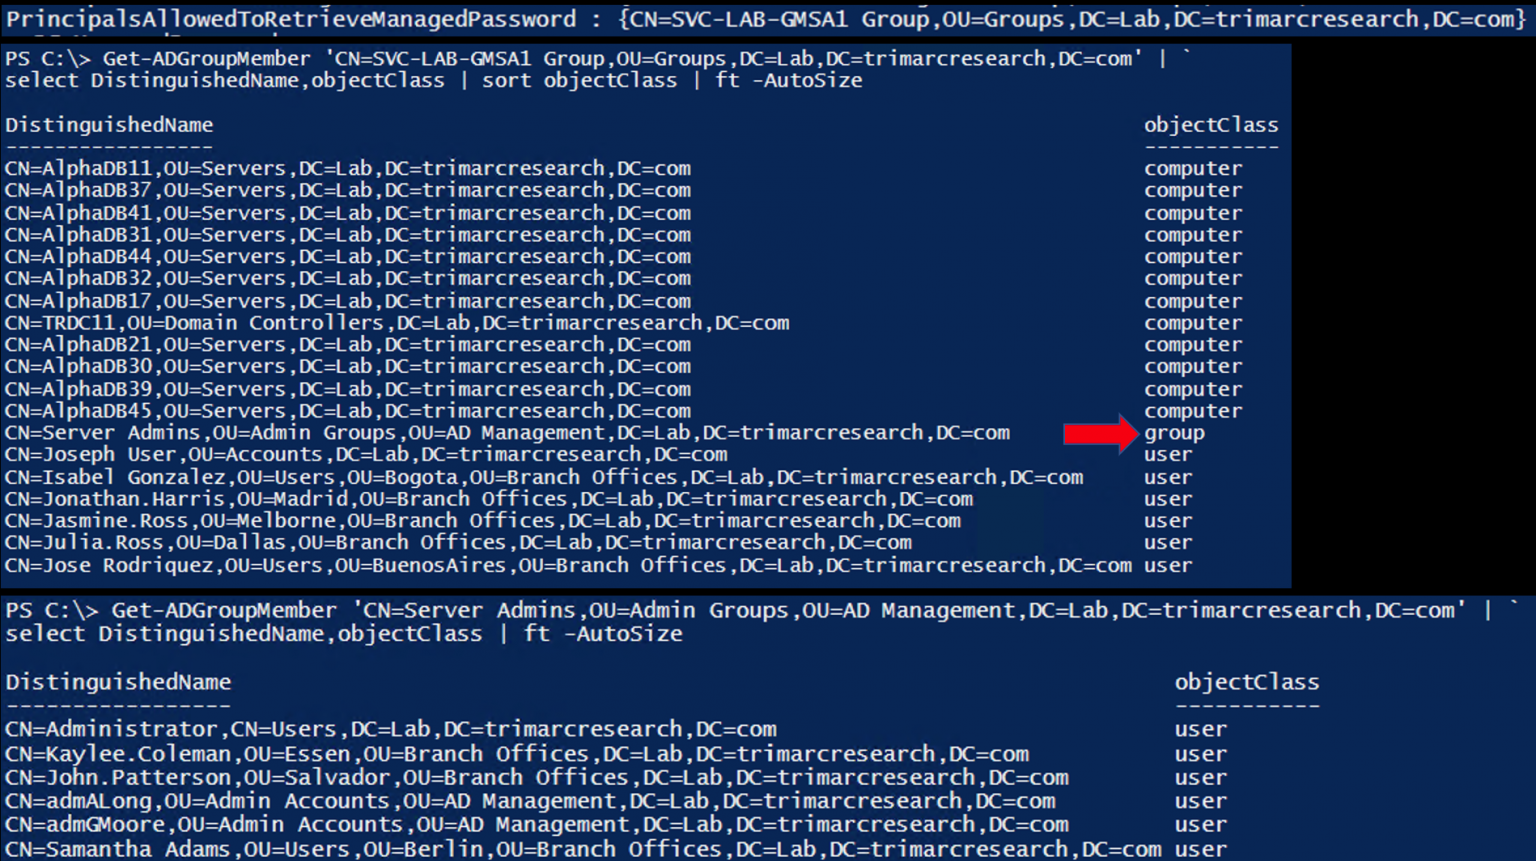
\includegraphics[width=0.75\linewidth]{msdsgrp.png}
    \caption{Enter Caption}
    \label{fig:placeholder}
\end{figure}

The msDS-GroupMSAMembership (PrincipalsAllowedToRetrieveManagedPassword) attribute contains a group called “SVC-LAB-GMSA1 Group”. This attribute controls who can request and receive the clear-text password.

When enumerating the membership of the group “SVC-LAB-GMSA1 Group” there are computers, users, and another group (“Server Admins”), so lets check the members of that group.

\begin{figure}
    \centering
    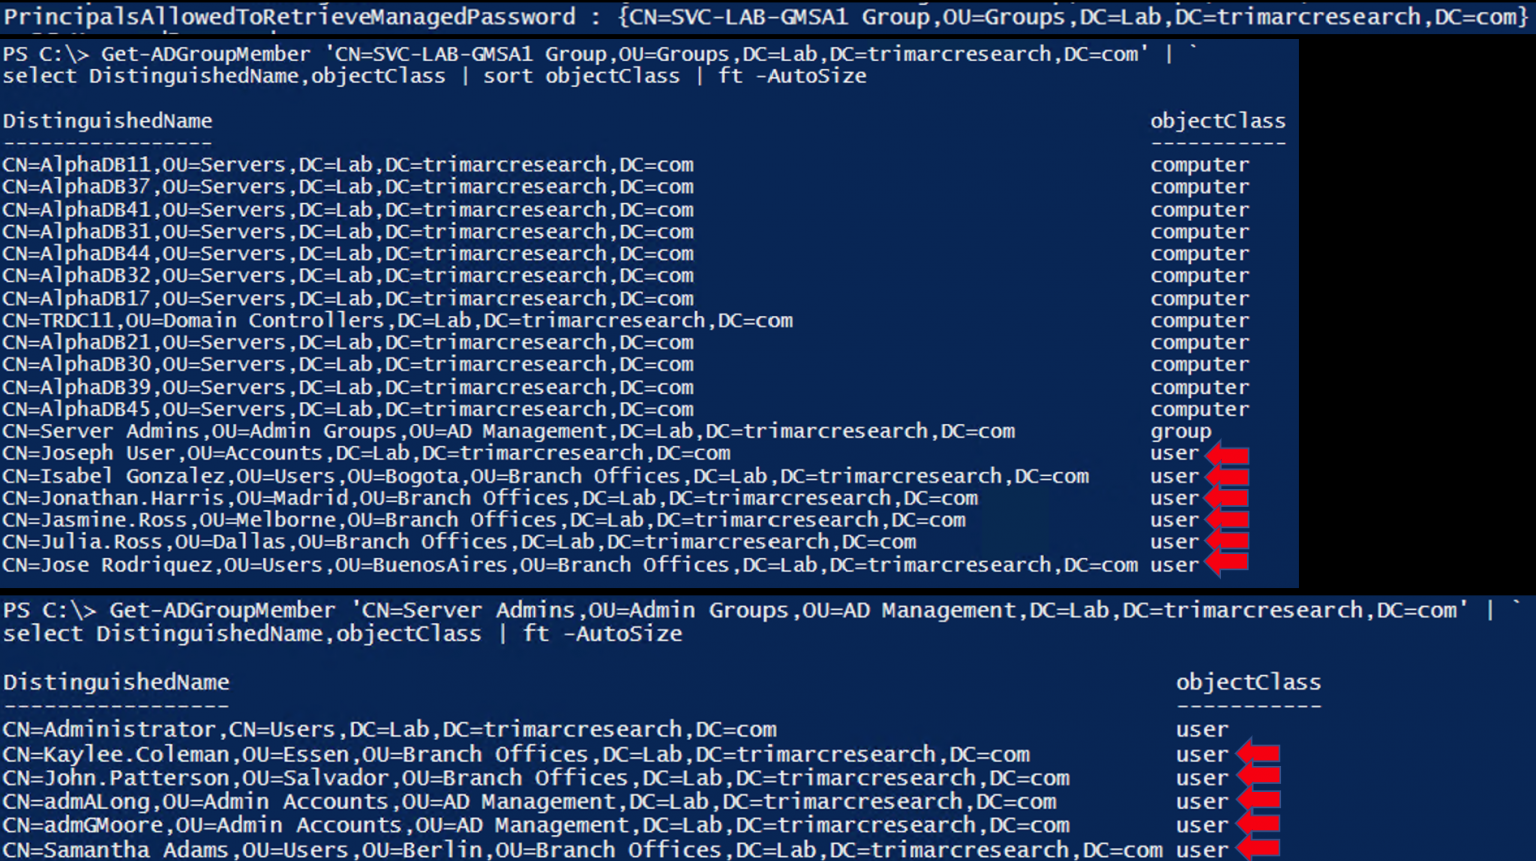
\includegraphics[width=0.75\linewidth]{gsma.png}
    \caption{Enter Caption}
    \label{fig:placeholder}
\end{figure}

Now we have a list of all accounts that can get the clear-text password for the GMSA. There are 11 user accounts with that ability and 9 of those look like regular user accounts (hint: they are!). That’s a big problem.
Compromise one of those and the GMSA account is compromised and since it’s a member of the Administrators group in the domain, we own the domain.

Once we compromise a user (or computer!) account that has the ability to pull the clear text password. (PrincipalsAllowedToRetriveManagedPassword), we can request that using the Microsoft PowerShell cmdlet Get-ADServiceAccount.

We can leverage the PowerShell cmdlet Get-ADServiceAccount to get the clear-text password data for the GMSA (attribute msds-ManagedPassword). Using the DSInternals module (ConvertTo-NTHash), we can convert the clear-text password blob to the NT hash.

\begin{figure}
    \centering
    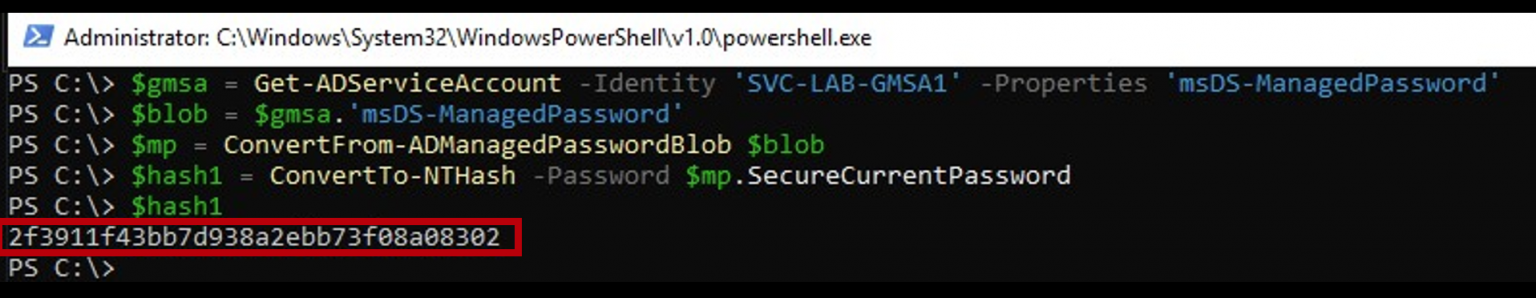
\includegraphics[width=0.75\linewidth]{nthash.png}
    \caption{Enter Caption}
    \label{fig:placeholder}
\end{figure}

If the account we are able to compromise is the computer account, we need to run these commands as SYSTEM on the computer. This method would be used if we’re able to get admin/SYSTEM rights on the server with rights to pull the GMSA password, but the GMSA is not running under the context of a service (so running Mimikatz doesn’t help since the GMSA creds aren’t in memory).

Here I use PSEXEC to spawn a command shell running under the context of the local SYSTEM account. Once running as SYSTEM, we can perform the same action as shown above. The computer account has the right to pull the password, but not a user on that computer, so I elevate to SYSTEM which then interacts with AD as the associated AD computer account. Now I can get the GMSA password.
\begin{figure}
    \centering
    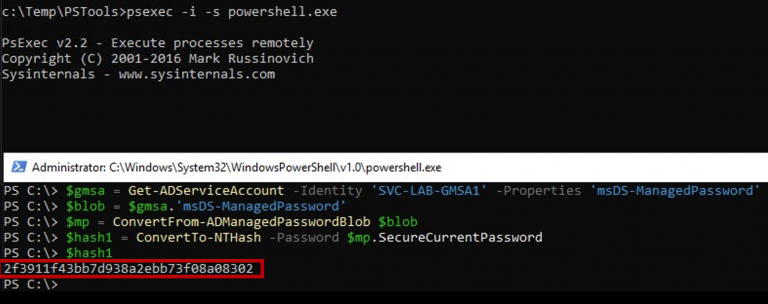
\includegraphics[width=0.75\linewidth]{gsmapass.png}
    \caption{Enter Caption}
    \label{fig:placeholder}
\end{figure}

Next step I perform in the lab is to to confirm that the NT password hash that DSInternals provides matches that in Active Directory.
I use the DSInternals command Get-ADReplAccount to get the AD password hash and can confirm that the password hash pulled from the GMSA is the same as that gathered from AD.
\begin{figure}
    \centering
    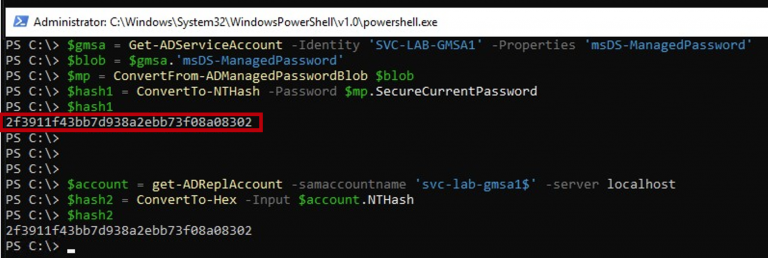
\includegraphics[width=0.75\linewidth]{dsintcmd.png}
    \caption{Enter Caption}
    \label{fig:placeholder}
\end{figure}


Mitigation

Determine rights actually required and ensure the only the required, limited rights apply to the GMSA.
Don’t add to AD privileged groups unless the servers the GMSAs are used on are limited to Tier 0 (Domain Controllers).
Limit GMSA access \& location (especially if privileged).
